\subsection{Diseño de la Fuente de Alimentación Lineal}
\bigskip 

En líneas generales, todo el amplificador estará alimentado por cuatro rieles, dos de alta tensión y dos de baja. Los rieles de altas serán suministrados por una fuente lineal mientras que para los de bajas, se reducirá la tensión de los rieles altos con una fuente conmutada. En esta sección se detallara el diseño de la fuente lineal. La misma consiste esencialmente de tres bloques:

\begin{itemize}
\item Transformador 220/36+36
\item Rectificador de onda completa
\item Divisor capacitivo 
\end{itemize}

El transformador reduce de 220$V_{rms}$ a 72$V_{rms}$, es decir, tensión pico de $72V_{rms}*\sqrt{2}=101.82V$.

Para el rectificador de onda completa se usaron diodos 6A10 en paralelo con capacitores de $100nF$ para reducir ruido. La caída en los diodos es de aproximadamente $0.7V$, reduciendo la tensión a la salida de este bloque a $101.82V-2*0.7V=100.4V$

Finalmente para el divisor capacitivo, se colocaron dos hileras de capacitores en paralelo, dando un divisor de $2200{\mu}F*4=8800{\mu}F$. El punto medio del divisor toma la tension de tierra, y los otros, $\pm50.2V$.


\begin{figure}[H]
\centering
\centerline{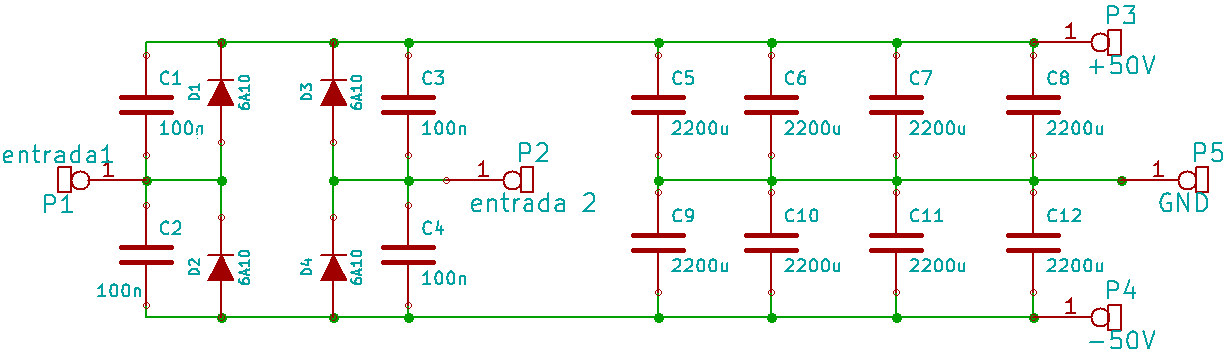
\includegraphics[scale=0.4]{img/esquema_fuente_lineal.png}}
\caption{Esquema de la fuente lineal}
\label{esquema_fuente_lineal} 
\end{figure}
\medskip
\subsubsection*{Ripple}

Para calcular el factor de rizado $F_r=\frac{V_{ca}}{V_{cd}}$ vamos a separar los casos entre el riel alto y el bajo, porque no ven la misma carga.

El riel alto ademas de ver el amplificador, alimenta la fuente de switching, así que las impedancias de entrada quedan en paralelo, empeorando el factor de ripple. Aproximadamente la impedancia de entrada de la switching son $500\ohm$, despreciando todo menos la resistencia en serie que se ve del bobinado del relé y el bobinado del primario. Luego, $500\ohm$ en paralelo con la resistencia de entrada simulada del amplificador $1.8k\ohm$ es aproximadamente $400\ohm$.Ve también un capacitor de $220{\mu}F$.
Por tanto, el factor de rizado queda:

\[
	F_r=\frac{1}{\sqrt{3}(4fRC-1)}$$
$$	F_r=\frac{1}{\sqrt{3}(4\times 50Hz\times 400\ohm\times (8800+220){\mu}F-1)}$$
$$	F_r=0.00046
\]

El riel bajo ve aproximadamente $R_i=\frac{-50V}{-25mA}=2k\ohm$, valor de corriente obtenido por simulación sin señal. Ve también un capacitor de $220{\mu}F$.
Por tanto, el factor de rizado queda:

\[
	F_r=\frac{1}{\sqrt{3}(4fRC-1)}$$
$$	F_r=\frac{1}{\sqrt{3}(4\times 50Hz\times 2k\ohm\times (8800+220){\mu}F-1)}$$
$$	F_r=0.00016
\]

Para el peor caso de carga, es decir con una entrada de $V_i=1V_{rms}$, la carga vista será $R_i=\frac{-50V}{-4A}=12.5\ohm$ y $F_r=0.026$ en el pico del semiciclo negativo. Este caso será sumamente inusual de ver.
\medskip
\subsection{Fuente Conmutada}

Para este tipo de fuente utilizaremos la topología Flyback con dos salidas, debido a su sencillez y bajo costo, su esquema puede observarse en la Figura~\ref{topo_flyback}. se Utilizaron dos bobinas de salida para generar 20V c/u; aprovechando el aislamiento galvánico generado por las bobinas acopladas se conectaron de forma tal de obtener dos bornes de $\pm 20V$, como se observa en la Figura~\ref{conmutada_basica} . Para controlar el ancho del pulso que activa el mosfet se utilizo un TL494, con un divisor a la salida para reescalar a una tension que el integrado pueda manejar fácilmente.

\begin{figure}[H]
\centering
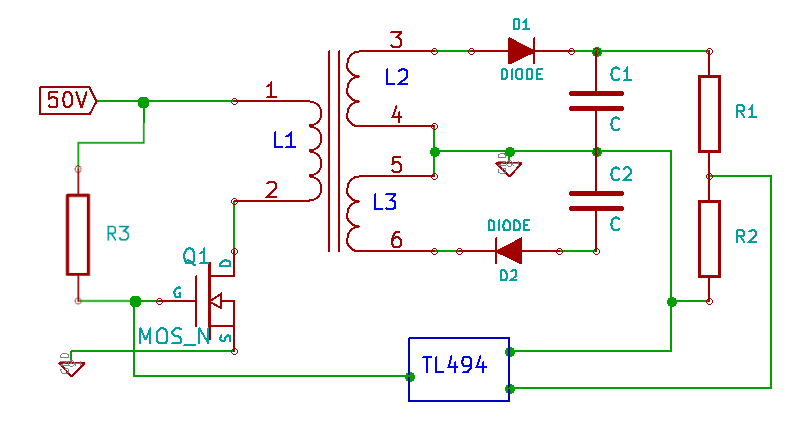
\includegraphics[width=0.85\textwidth]{img/conmutada_basica.png}
\caption{Esquema  basico fuente conmutada.}
\label{conmutada_basica}
\end{figure}
\medskip
\subsubsection{Controlador}
\medskip
Se utilizó el circuito integrado TL494 como circuito de control de la fuente conmutada. El método de control es mediante la modulación del ancho de pulso, las características y funcionalidades de este integrado se explican en la Sección~\ref{TL494}. Para facilitar la comparación de tensiones se utilizo la referencia de 5V integrada en el TL494, por lo tanto se definieron: R1=$33\kohm $ y R2=$8.2\kohm$ para que la salida se estabilice en 20V. Este sensado de tension se aplico a ambos comparadores del integrado, para poder utilizar ambas salidas simultáneamente y exigir menor corriente a cada una.
\medskip
\subsubsection{Llave conmutadora}
\medskip
Esta se implemento con un mosfet que pudiera soportar las corrientes que circularían por el devanado primario. Para controlar la tension de gate del transistor se utilizo una resistencia de $3.3\kohm$ en el colector de los transistores de salida del TL494, por los que pueden circular 400mA, siendo la resistencia utilizada más que suficiente para saturarlos. Por lo tanto, el gate del mosfet puede ir desde los 50V de alimentación hasta los 1.3V, debido al $V_{CE}$ de los transistores del TL494. Teniendo en cuenta los picos de tension que se generan en las conmutaciones, se protegió el transistor con un snub.
Se implementó un circuito con relé para retrasar el paso de corriente por los inductores, de modo de permitir que el TL494 se encienda primero. De otra forma, el TL494 encendía despues, no funcionaba de PWM en el transitorio inicial y se quemaba el MOSFET. El circuito de retraso se implementó con un capacitor grande y un BC548, cuya juntura base-emisor esté en paralelo con el capacitor. Así el delay viene dado por lo que tarda en cargarse el capacitor, y es de aproximadamente 3 segundos, valor que permite el correcto funcionamiento de la fuente. 

\medskip
\subsubsection{Determinación de la inductancia del primario}
\medskip
La fuente flyback se diseño para operar en modo discontinuo. Para asegurar esto, la 
inductancia del bobinado primario($L_P$) necesita estar limitada a un valor máximo.
Por lo tanto, debe determinarse este valor a carga máxima, para esto se requiere definir la
potencia de entrada como:
$$
P_{in}= \frac{P_{out}}{\eta}
$$
Donde $\eta$ es la eficiencia del inductor.

En una inductor/transformador flyback se puede asumir que este valor es cercano al $80\%$, y como la potencia máxima de salida $P_{out}$ esta definida a 40W (2A $\times$ 20V).Por lo tanto $P_{in}$=50W.

La potencia de entrada también puede ser definida como el producto de la energía almacenada($E_{in}$) el campo magnético y para la frecuencia de funcionamiento de nuestra fuente vale que:

\begin{equation}
P_{in}= E \times fs = \frac{Lp \times I_{pk}^2}{2} \times fs \label{potencia_entrada_L}
\end{equation}

Este razonamiento requiere que la inductancia del primario sea definida, pero para ello sería necesario conocer el pico de corriente $I_{pk}$. Este pico de corriente puede ser definido como:
$$
I_{pk}=V_{in(min)} \times \frac{t_{ON(max)}}{L_P}
$$

donde $V_{in(min)}$ es el mínimo voltaje de entrada y el $t_{ON(max)}$ es el máximo tiempo en un nivel alto de tensión. Por lo tanto, para limitar la inductancia del primario para asegurar operación discontinua, la inductancia máxima es determinada por:

\begin{equation}
L_P \leq V_{in(min)} \times \frac{t_{ON(max)}}{I_{pk}}= \frac{V{in(min)}}{Ipk} \times \delta_{max} \times T_s \label{L_p}   
\end{equation}

donde  $\delta_{max}$ es el máximo duty cicle alcanzado por el TL494 (45$\%$), $T_s$ el período de la frecuencia de funcionamiento de la fuente switching($T_s =12.5\E{-6}$ a una frecuencia de operación de 80kHz), una tensión mínima $V_{in(min)}$ =46V y una $I_{pk}$= 4,83A.
Combinando las ecuaciones \ref{L_p} y \ref{potencia_entrada_L} es posible determinar la máxima inductancia del primario:
$$
L_{P(max)} = \frac{V_{in(min)}^2 \times \delta_{max}^2 \times Ts}{2 \times P_{in(max)}} = 54\mu H
$$

\medskip
\subsubsection{Selección del núcleo}
\medskip

Se utilizara el método de calcular el producto de área para determinar el tamaño del núcleo del inductor, definiendo como:
$$
Ap= {\left( \frac{  2 \times E \E{4}}{Bm \times Ku \times Kj} \right) } ^{ 1.14}
$$
donde:
\begin{list}{ }
\item Kj = coeficiente de densidad de corriente.
\item Bm =máxima densidad  de flujo 
\item Ku = factor de utilización de ventana 
\item Ap = producto de área 
\item E = Energía Acumulada = $ L_P \times \frac{I_{pk}^2 }{2}$ 
\item
\end{list}

Aunque esta ecuación empírica es utilizada para núcleos con un único inductor. Para modificarla se debe suponer que el secundario utilizará una energía similar al primario, por lo tanto:
$$
A p= 2 \times {\left( \frac{  2 \times E \E{4}}{Bm \times Ku \times Kj} \right) } ^{ 1.14}
$$
Para valores de Bm=0.32T  Kj=500 y Ku=0.3. Obtenemos un Ap=4134$mm^4$
Por lo tanto, y por cuestiones de disponibilidad usamos el núcleo E30/15/7 el cual tiene un Ap= 4800 $mm^4$

\subsubsection{Determinación del número de espiras del primario}

Una vez seleccionado el núcleo es elegido el mínimo entrehierro(Ig) requerido se calcula como:
$$
Ig= \frac{1.26 \times L_{P(max)} \times Ipk^2}{(Ac*Bm^2)}
$$

Donde Ac es el área efectiva del núcleo, para nuestro caso Ac=0.6 $cm^2$. Por lo tanto, el mínimo entrehierro será de Ig=0.25mm

Como este entrehierro no es comercial debimos implementarlo manualmente. Por ende los siguientes cálculos fueron realizados solo como una aproximación.
Siguiendo con el razonamiento:
$$
Np= 1000 \times \sqrt{\frac{L{P(max)}}{Al}}
$$
donde asignamos un valor característico al Al de 250 mH obteniendo: Np=15
\medskip
\subsubsection{Determinación del número de espiras del secundario}

Para garantizar funcionamiento en modo discontinuo en la máxima corriente de carga, es necesario limitar la inductancia de los devanados secundarios a un cierto valor máximo. La pendiente de corriente negativa es:
$$
\frac{di}{dt}= \frac{Is}{t_{fly}} = \frac{V_o+V_D}{L_S}
$$
donde:
\begin{list}{ }
\item  Is es la corriente pico del secundario.
\item $t_{fly}$ es el tiempo de caida. 
\item $V_o$ es la tensión de salida. 
\item $V_D$ es la tensión de caída en el diodo de salida.
\item $L_S$ la inductancia del secundario.
\item
\end{list}

El duty cicle de la fuente se define como:
$$
\delta_r= \frac{t_{fly}}{Ts}
$$

y la corriente de carga $I_o$ esta relacionada con el pico de corriente en el secundario
como:
$$
Is=\frac{2 \times I_o }{\delta_r}
$$

Combinando estas últimas 3 ecuaciones obtenemos que:
$$
L_S \leq \frac{\delta_r^2 \times (V_o + V_D) \times Ts}{2 \times I_o} =12.97\mu H
$$

Por último:
$$
Ns= 1000 \times \sqrt{\frac{Ls}{Al}}=8
$$
\medskip
\subsubsection{Circuito Implementado}

Como se observa en la Figura~\ref{conmutada_cir} se agregaron a la configuración explicada del TL494 un rele que otorga un delay entre el encendido de cada tipo de fuente, otorgando a la lineal tiempo más que suficiente de cargar sus capacitores de salida.

\begin{figure}[H]
\centering
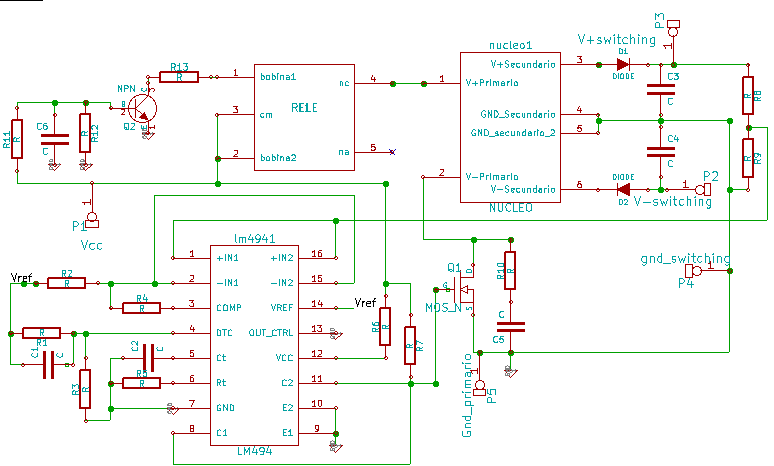
\includegraphics[width=0.90\textwidth]{img/cir_conmutada.png}
\caption{Esquema  de la fuente conmutada, implementada.}
\label{conmutada_cir}
\end{figure}

\medskip
